\section{Figures and Tables}
\label{sec:figures}

Figures and tables carry evidence; captions carry meaning. A common
mistake is a one-line caption like ``Results'' under a plot with three
unlabelled axes. \Cref{fig:latency} shows a better pattern: the caption
states what is plotted, the axes, and the one-sentence takeaway, so the
figure is understandable even if a reader skips the surrounding text.

\begin{figure}[htbp]
  \centering
  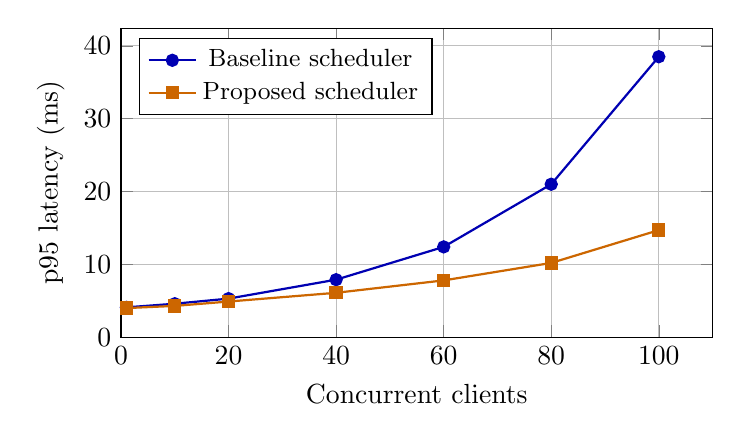
\begin{tikzpicture}
    \begin{axis}[
        width=0.75\linewidth,
        height=5.5cm,
        xlabel={Concurrent clients},
        ylabel={p95 latency (ms)},
        xmin=0, xmax=110,
        ymin=0,
        grid=major,
        legend pos=north west,
        legend style={font=\small},
      ]
      \addplot[thick, mark=*, color=blue!70!black] coordinates {
        (1,4.1) (10,4.6) (20,5.3) (40,7.9) (60,12.4) (80,21.0) (100,38.5)
      };
      \addlegendentry{Baseline scheduler}
      \addplot[thick, mark=square*, color=orange!80!black] coordinates {
        (1,4.0) (10,4.3) (20,4.9) (40,6.1) (60,7.8) (80,10.2) (100,14.7)
      };
      \addlegendentry{Proposed scheduler}
    \end{axis}
  \end{tikzpicture}
  \caption{95th-percentile request latency versus number of concurrent
  clients, for the baseline round-robin scheduler and the proposed
  load-aware scheduler (\cref{sec:algorithms}). The proposed scheduler
  degrades more gracefully under load. \emph{(Illustrative numbers, not
  real measurements --- in your own report this caption should also
  point to the section describing your experimental setup.)}}
  \label{fig:latency}
\end{figure}

\begin{tipbox}
Every figure and table needs: a caption that stands on its own, labelled
axes with units, a legend if there is more than one series, and a
reference from the body text (``\texttt{\textbackslash cref\{fig:latency\}}
shows\ldots''). A figure the text never mentions is a figure the reader
will skip.
\end{tipbox}

\subsection{Tables}
Use tables for precise numbers the reader may want to look up; use
figures for trends and shapes. \Cref{tab:comparison} is a minimal
example using the \texttt{booktabs} package, which gives cleaner
horizontal rules than the default \LaTeX{} table style (avoid vertical
rules and ``double'' borders --- they add visual noise, not information).

\begin{table}[htbp]
  \centering
  \caption{Comparison of the two schedulers at 100 concurrent clients.
  Throughput in requests per second; latency in milliseconds.}
  \label{tab:comparison}
  \begin{tabular}{@{}lrrr@{}}
    \toprule
    Scheduler & Throughput (req/s) & p50 latency & p95 latency \\
    \midrule
    Baseline (round-robin) & 8{,}120  & 9.8 ms  & 38.5 ms \\
    Proposed (load-aware)  & 11{,}940 & 6.1 ms  & 14.7 ms \\
    \bottomrule
  \end{tabular}
\end{table}

\begin{pitfallbox}
  Do not screenshot a table from a spreadsheet or a terminal. Rebuild it
  natively in \LaTeX{} (as above) so that fonts, alignment, and decimal
  points match the rest of the document.
\end{pitfallbox}

\subsection{Placement and referencing}
Let \LaTeX{} place floats (\texttt{htbp}) rather than fighting it with
exact positions; refer to figures/tables by label
(\verb|\cref{fig:latency}|) rather than by position (``the figure
above''), since positions shift as the document is edited.
